\documentclass[a4paper, 12pt]{article}
\usepackage{graphicx} % For including figures
\usepackage{amsmath}  % For mathematical symbols and formulas
\usepackage{hyperref} % For hyperlinks
\usepackage{geometry} % For margins
\geometry{margin=0.55in} % For including images (optional)
\usepackage{xcolor}
\usepackage{setspace}
\usepackage{titlesec}
\usepackage{fancyhdr}
\usepackage{ulem}
\usepackage{cite}
\usepackage{float}
\usepackage{subcaption}


\renewcommand{\headrulewidth}{0pt}


\definecolor{grun}{RGB}{60, 100, 180}

\hypersetup{
    colorlinks=true,
    citecolor=grun,
    linkcolor=black,
    urlcolor=grun,  % Keep color for clickable links
    pdfborder={0 0 0}  % Remove borders around links
}

\renewcommand\ULdepth{1pt}


\onehalfspacing

\titleformat{\section}
  {\normalfont\Large\bfseries} % Keeps the section title normal
  {\textcolor{grun}{\thesection}} % Change number appearance (color, style)
  {1em}{} 

% Customize subsection numbers
\titleformat{\subsection}
  {\normalfont\large\bfseries} % Title formatting
  {\textcolor{grun}{\thesubsection}} % Red subsection number
  {1em}{}

% Customize subsubsection numbers
\titleformat{\subsubsection}
  {\normalfont\normalsize\bfseries} % Title formatting
  {\textcolor{grun}{\thesubsubsection}} % Green subsubsection number
  {1em}{}

  \pagestyle{fancy}
\fancyhf{} % Clear default headers/footers
\fancyfoot[C]{\textcolor{grun}{\thepage}}
  
\begin{document}


\begin{titlepage}
    \centering 
    
    \vspace*{2cm}
    
{\LARGE \textbf{\textcolor{grun}{Content Comparison:} How Disney+ and}} 

\vspace{0.5cm} % Adds vertical space after "and"

{\LARGE \textbf{Netflix Differ in \textcolor{grun}{Age Ratings} and \textcolor{grun}{Quality}}} \\[3cm]

    {\Large Application Report for Master of Science in Data Science}\\[1cm]
      {\large Submitted to \textbf{\href{https://statistik.tu-dortmund.de/en/}{TU Dortmund's Faculty of Statistics}}}\\[0.5cm]

    % 
\includegraphics[width=0.1\textwidth]{tu.png}
    % \hspace{15pt}
    % 
\includegraphics[width=0.3\textwidth]{stat.png}
    
    \vspace{3cm}
    \textcolor{grun}{\textbf{Author:}}\\
    Mohammad Karbalaee Shabani \\[0.5cm]
    
    \textcolor{grun}{\textbf{Date:}}\\
    \today \\[2cm]

    \textbf{Source Code:}\\
    \vspace{0.15cm}
    \href{https://github.com/mohammadkarbalaee/Movies-on-Netflix-Prime-Video-Hulu-and-Disney}{GitHub Repository} \\[0.1cm]
    \href{https://colab.research.google.com/drive/1ndNb2C8GhkVdQ8_PwA0n4-C5B5k3smSz?usp=sharing}{Notebook on Colab}
    
\end{titlepage}

\pagenumbering{gobble}
\tableofcontents

\newpage

\pagenumbering{arabic} % Start Arabic numbering from this page
\setcounter{page}{1}
\section{Introduction}

Streaming platforms have revolutionized entertainment, offering convenience and vast content libraries. Among the most popular services, Disney+ is often viewed as a family-friendly platform, while Netflix is known for its diverse content, spanning genres from comedies to mature dramas.

\subsection{Key Questions}

Despite their reputations, both platforms cater to broader audiences. Disney+ features franchises like Marvel and Star Wars, which appeal beyond children, while Netflix includes family-friendly titles. This raises two critical questions:
\begin{itemize}
    \item Does Disney+ predominantly feature content with lower age restrictions?
    \item Are Netflix movies generally of higher quality, based on Rotten Tomatoes scores?
\end{itemize}

\subsection{Relevance of the Analysis}

These questions have practical implications. Families need guidance on selecting platforms with appropriate content, while movie enthusiasts seek high-quality films. Streaming services can also use such insights to refine their content strategies and target audiences more effectively. \cite{Nielsen2021}

\subsection{Approach and Report Structure}

This report uses the dataset of movies from Disney+ and Netflix \cite{dataset}. First, a descriptive analysis explores age ratings and Rotten Tomatoes scores. Then, hypothesis tests evaluate whether observed differences are statistically significant.

The report is organized as follows:
\begin{itemize}
    \item \textbf{Section 2: Problem Description} - Explains the problem and dataset.
    \item \textbf{Section 3: Methods} - Outlines statistical methods and tests.
    \item \textbf{Section 4: Evaluation} - Presents descriptive and inferential analysis results.
    \item \textbf{Section 5: Summary and Discussion} - Concludes with findings and implications.
\end{itemize}


\section{Problem Description}

To address the research questions, we will first conduct a thorough exploratory data analysis to extract meaningful insights from the dataset. Based on these initial findings, we will formulate hypotheses and develop preliminary claims regarding the differences between Disney+ and Netflix. These claims will then be subjected to rigorous statistical validation using appropriate methods, such as the t-test, to ensure their reliability and accuracy. Through this process, we aim to draw robust conclusions and provide answers to the proposed research questions.

\subsection{Dataset Overview}

This section provides a foundational understanding of the dataset, outlining its structure and key variables to set the stage for further analysis.

\subsubsection{Data Source and Collection}

The dataset comprises data that was scraped from multiple streaming platforms, including Netflix, Disney+, Hulu, and Prime Video. The scraping process provided a comprehensive list of movies available on these platforms, capturing key metadata. This method ensured a systematic and extensive collection of data from publicly accessible information.



\subsubsection{Dataset Variables and Their Characteristics}

The dataset contains \textbf{9515 records} and represents movies from major streaming platforms. This dataset consists of 11 columns with various data types. Most columns, such as \texttt{ID}, \texttt{Year}, and platform indicators (\texttt{Netflix}, \texttt{Hulu}, etc.), are integers (\texttt{int64}). The \texttt{Title} column stores movie names as objects and generally does not require processing. However, the \texttt{Age} and \texttt{Rotten Tomatoes} columns, also stored as objects, need to be converted to appropriate formats for analysis and statistical testing. \textbf{Figure~\ref{fig:datatable}} in the appendix shows the first few rows of the dataset.


\subsubsection{Missing Values}

The dataset contains missing values in two key columns:

\begin{itemize}
    \item \textbf{Age}: 
    \begin{itemize}
        \item \textbf{Missing Values}: 4,177 entries
        \item \textbf{Percentage}: 43.9\%
    \end{itemize}
    This is a significant proportion of the dataset, suggesting that nearly half of the records lack age ratings. Since this variable is crucial for analyzing age suitability, appropriate handling of these missing values is necessary. Options include imputation (e.g., replacing missing values with the most frequent category) or excluding these rows, depending on the analysis requirements.

    \item \textbf{Rotten Tomatoes}:
    \begin{itemize}
        \item \textbf{Missing Values}: 7 entries
        \item \textbf{Percentage}: 0.07\%
    \end{itemize}
    The number of missing values here is minimal and unlikely to affect the overall analysis significantly. These can either be imputed using the mean or median score or removed without substantial impact.
\end{itemize}


\section{Methods}
This section provides a detailed description of the advanced statistical methods used in the analysis, including their mathematical definitions and references to relevant literature. Basic concepts are assumed to be known and are not covered here.

\subsection{Missing Value Imputation}

The dataset contains 1,797 Netflix movies and 197 Disney+ movies with missing \texttt{Age} values, totaling approximately 2,000 records. Dropping these entries would result in a significant loss of valuable data, making this approach unsuitable. Therefore, imputing the missing values is necessary.
We applied both \textit{mode imputation} and \textit{KNN imputation} methods, and the analysis will demonstrate why KNN imputation proves to be the more effective approach.

\subsubsection{Ordinal Encoding of Age Variable}

We applied \textit{ordinal encoding} to the \texttt{Age} variable to convert its categorical values (e.g., \texttt{7+}, \texttt{13+}, \texttt{18+}, \texttt{All}) into corresponding numeric values (e.g., \texttt{7}, \texttt{13}, \texttt{18}, \texttt{0}). This transformation was necessary to enable statistical analysis and visualization, as numerical data is required for most quantitative methods.

\textit{Ordinal encoding} is a technique used to convert categorical data with an inherent order into numerical form. In this case, higher values represent age suitability for older audiences, maintaining the natural hierarchy of the categories. \cite{von_eye1996categorical} This ensures that the encoded data reflects the meaningful relationships between age groups. \textbf{Figure~\ref{fig:age_encoding}} depicts the effect of this encoding.

\begin{figure}[H]
    \centering
    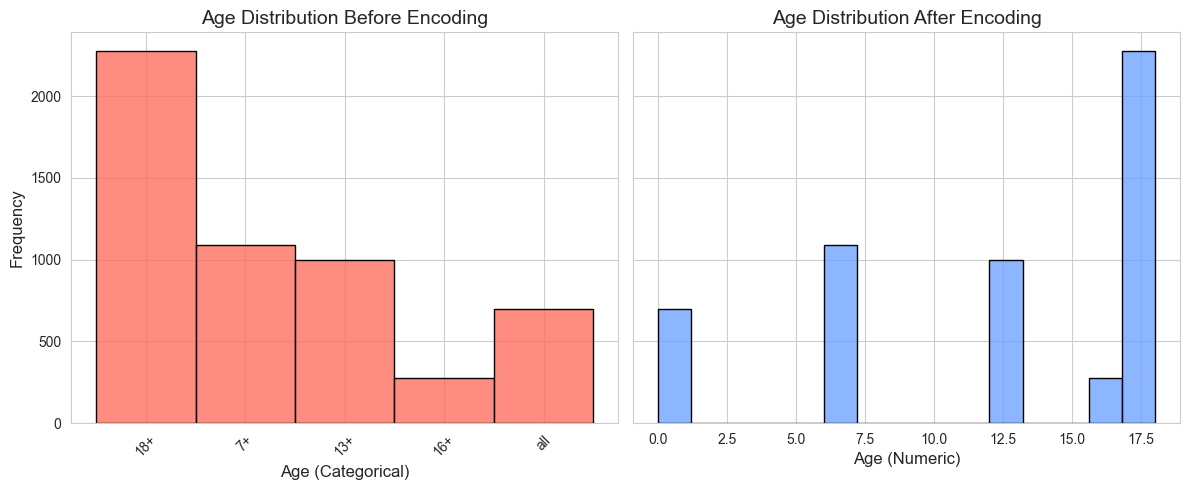
\includegraphics[width=\textwidth]{encode_age.png} % Replace 'output.png' with the actual filename
    \caption{Age Distribution Before and After Encoding}
    \label{fig:age_encoding}
\end{figure}

\subsubsection{Mode Imputation}

\textbf{Mode imputation} fails to handle the \texttt{Age} variable effectively, as seen in \textbf{Figure ~\ref{fig:mode_imputation}}. By replacing all missing values with the most frequent age (the mode), it creates an \textbf{artificial spike} in the distribution, leading to an unnatural concentration around a single age group. This oversimplifies the data and skews the original variability, as illustrated in the sharp peak in the \textit{After Mode Imputation} plot.

In contrast, the \textit{Before Mode Imputation} plot shows a natural spread across multiple age groups, reflecting a \textbf{multimodal distribution}. Mode imputation does not respect this diversity, making it unsuitable for data with multiple natural peaks. A more appropriate method, such as \textbf{KNN imputation} (refer to \autoref{appendix:knn}), maintains the original distribution by using similar records to estimate missing values.

\begin{figure}[H]
    \centering
    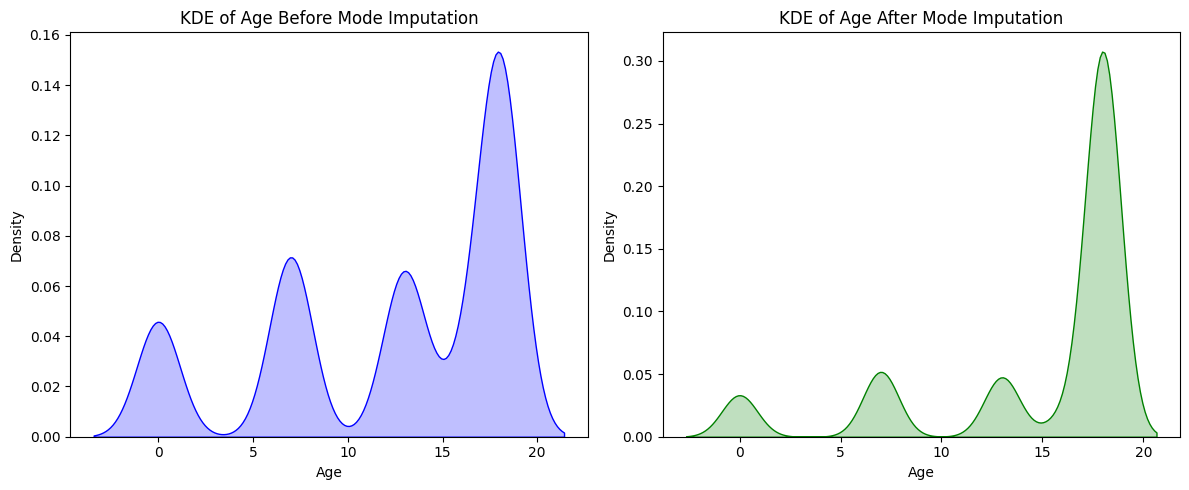
\includegraphics[width=\textwidth]{mode.png} % Replace 'output.png' with the actual filename
    \caption{Impact of Mode Imputation on Age Distribution: KDE Plot (refer to \autoref{appendix:kde})}
    \label{fig:mode_imputation}
\end{figure}

\subsubsection{KNN Imputation}

\textbf{Figure~\ref{fig:knn_imputation}} shows that KNN preserves the natural spread and multimodal peaks of the \texttt{Age} distribution. Unlike mode imputation, which created an artificial spike by concentrating missing values around a single age group, KNN imputation fills missing values based on similarity with neighboring records. This approach respects the original variability and maintains a more realistic distribution, as seen in the smooth, continuous curve of the \textit{After KNN Imputation} plot. This makes KNN a better choice for datasets with diverse categories, like age ratings.

\begin{figure}[H]
    \centering
    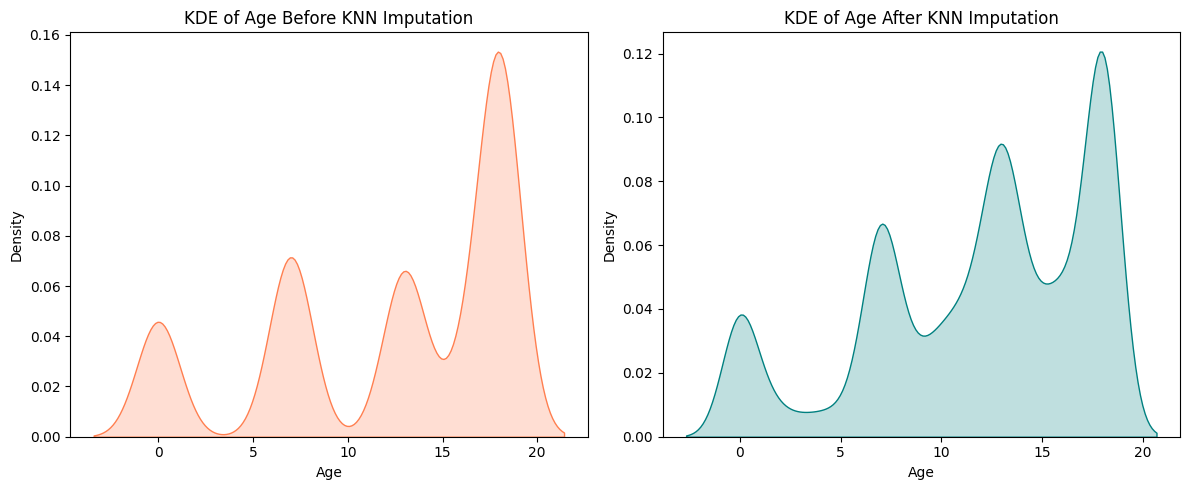
\includegraphics[width=\textwidth]{knn.png} % Replace 'output.png' with the actual filename
    \caption{KDE Plot of Age Distribution Before and After KNN Imputation}
    \label{fig:knn_imputation}
\end{figure}

\subsection{Visualization}

After handling the missing values, we calculated the \textbf{mean} and created \textbf{box plots} (refer to \autoref{appendix:box_plot}) for the \texttt{Age} and \texttt{Rotten Tomatoes} variables to visualize their distributions. These measures provide a summary of central tendency and variability.

\begin{figure}[H]
    \centering
    % First row: Age plots
    \begin{subfigure}[t]{0.48\textwidth}
        \centering
        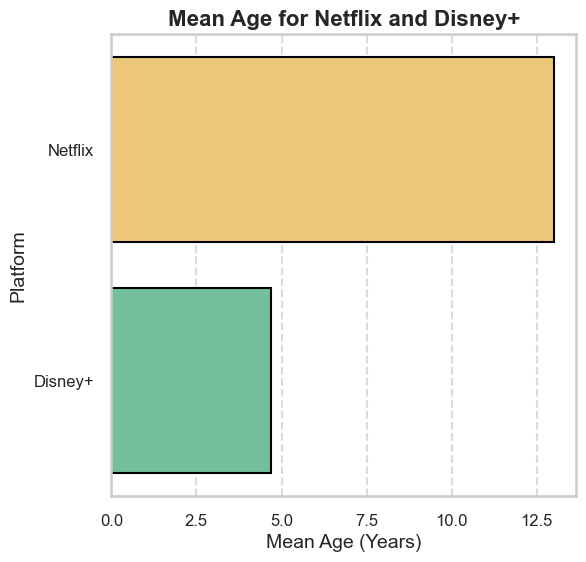
\includegraphics[width=\textwidth]{mean_age.png}
        \caption{Mean Age Ratings for Netflix and Disney+}
        \label{fig:mean_age}
    \end{subfigure}
    \hfill
    \begin{subfigure}[t]{0.48\textwidth}
        \centering
        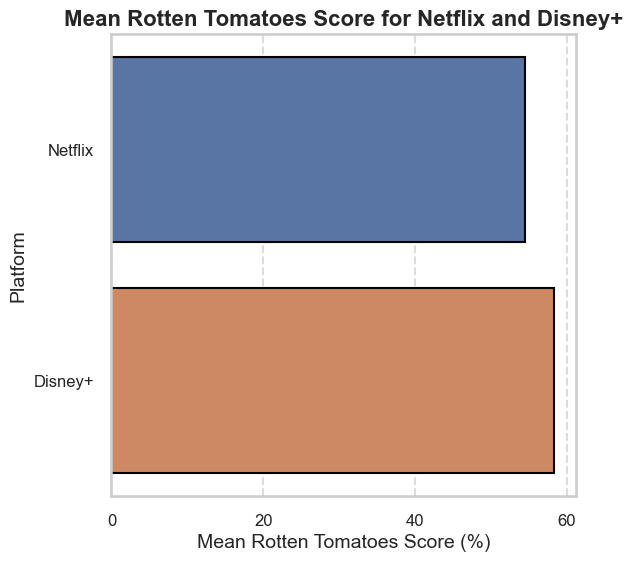
\includegraphics[width=\textwidth]{mean_tomato.png}
        \caption{Mean Rotten Tomatoes Scores for Netflix and Disney+}
        \label{fig:mean_tomato}
    \end{subfigure}

    \vspace{0.5cm} % Space between rows

    % Second row: Rotten Tomatoes plots
    \begin{subfigure}[t]{0.48\textwidth}
        \centering
        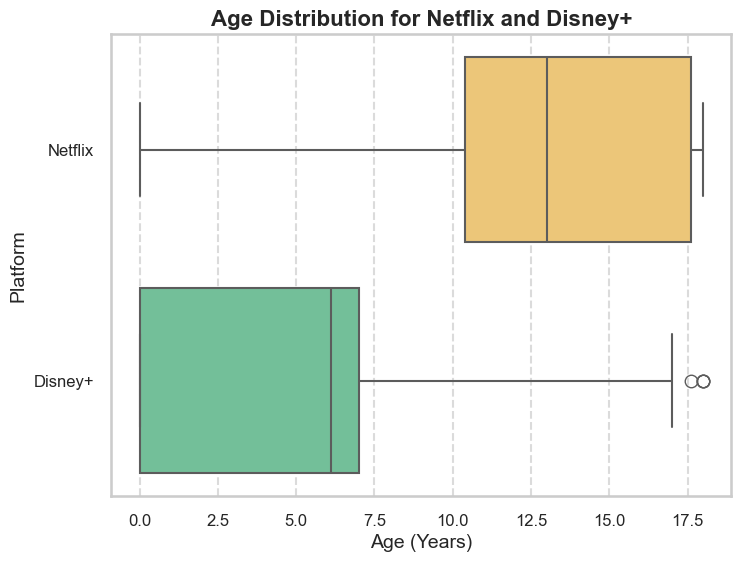
\includegraphics[width=\textwidth]{box_age.png}
        \caption{Age Distribution for Netflix and Disney+ (Box Plot)}
        \label{fig:box_age}
    \end{subfigure}
    \hfill
    \begin{subfigure}[t]{0.48\textwidth}
        \centering
        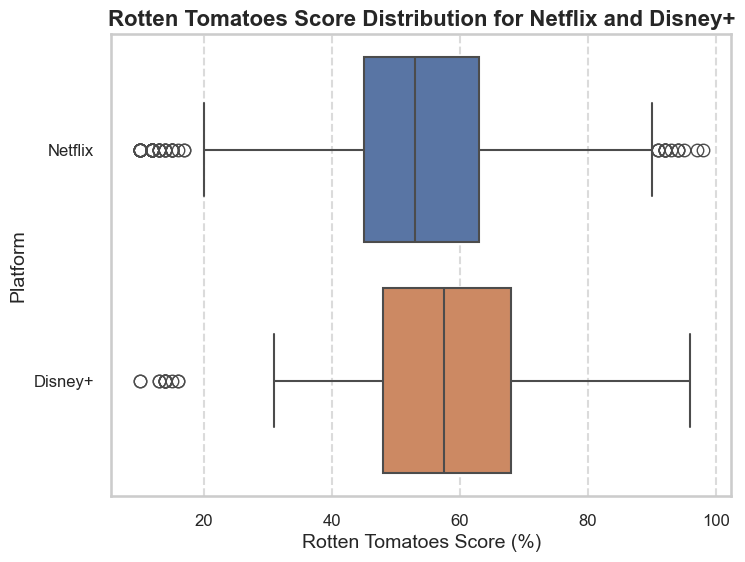
\includegraphics[width=\textwidth]{box_tomate.png}
        \caption{Rotten Tomatoes Score Distribution for Netflix and Disney+ (Box Plot)}
        \label{fig:box_tomato}
    \end{subfigure}

    \caption{Visualizations of Age Ratings and Rotten Tomatoes Scores for Netflix and Disney+}
    \label{fig:age_tomato_plots}
\end{figure}

\vspace{0.5cm}

\textbf{Figure~\ref{fig:mosaic_age}} features a mosaic plot regarding age categories. A \textbf{Mosaic Plot} is a visual tool used to analyze the relationships between categorical variables by representing them as proportional rectangles. Each rectangle's area corresponds to the frequency or relative frequency of a particular category combination, making it easy to compare distributions across groups. This plot is particularly useful for identifying patterns, dependencies, and disparities in data. In the given plot, it compares age ratings (0-7, 7+) across Disney+ and Netflix, highlighting which platform dominates specific age categories.

\begin{figure}[H]
    \centering
    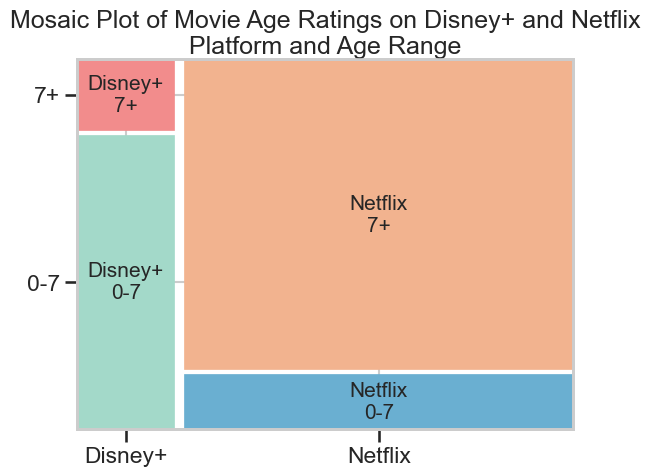
\includegraphics[width=0.5\textwidth]{mosaic.png} % Replace
    \caption{Mosaic Plot of Age Ratings Distribution Across Disney+ and Netflix}
    \label{fig:mosaic_age}
\end{figure}

\textbf{Figures~\ref{fig:rig_scatter_plots}} analyze Rotten Tomatoes scores for Netflix and Disney+. The Ridgeline Plot provides an overview of score distributions, highlighting density, central tendency, and variability, enabling clear platform comparisons by stacking multiple density plots. The Scatter Plot with Jitter complements this by displaying individual scores, reducing overlap with jitter to reveal clustering and outliers. Together, these visualizations offer both aggregated insights and granular details, providing a comprehensive understanding of the data. \cite{Waskom2021}

\begin{figure}[H]
    \centering
    % First row: Age plots
    \begin{subfigure}[t]{0.48\textwidth}
        \centering
        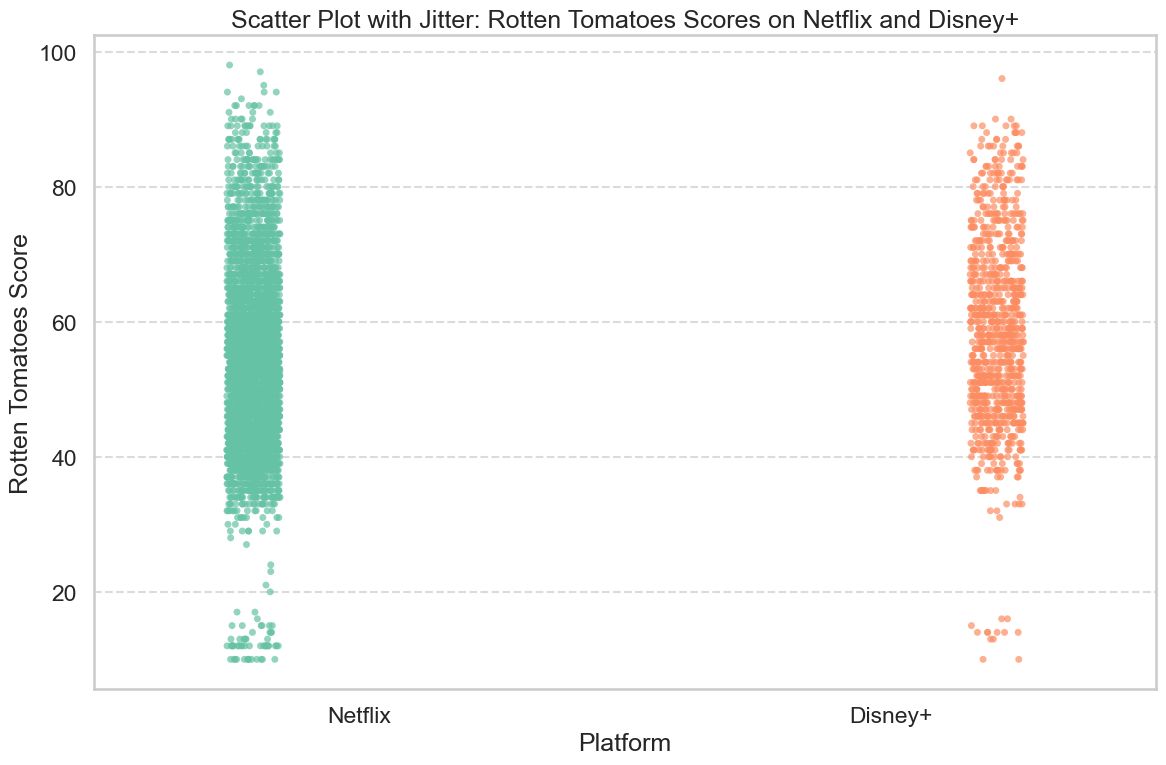
\includegraphics[width=\textwidth]{scatter.png}
        \caption{Scatter plot}
        \label{fig:scatter}
    \end{subfigure}
    \begin{subfigure}[t]{0.48\textwidth}
        \centering
        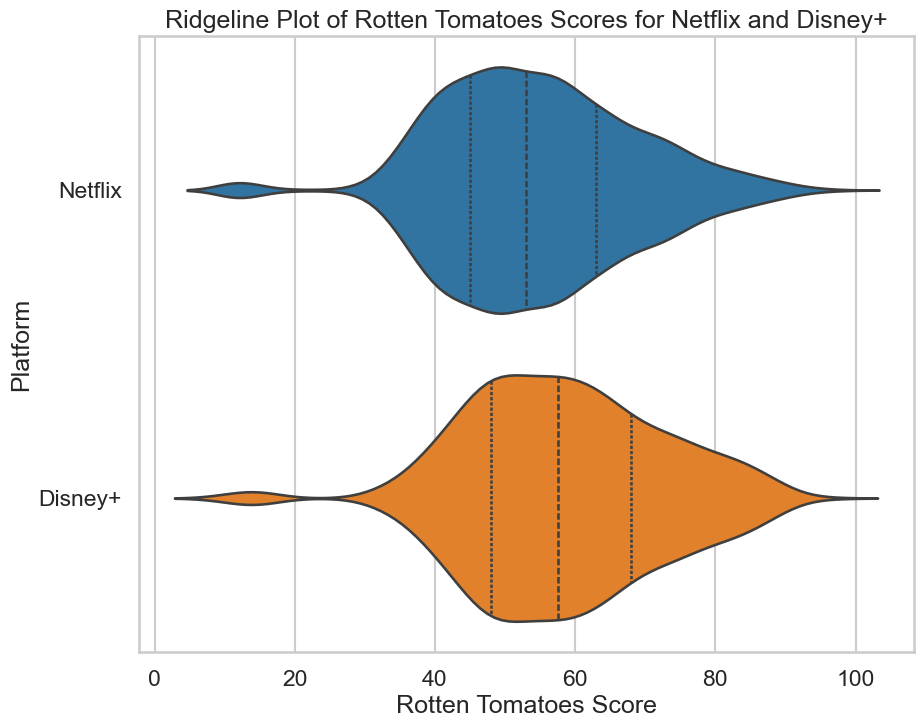
\includegraphics[width=\textwidth]{ridgeline.png}
        \caption{Ridgeline Plot}
        \label{fig:ridgeline}
    \end{subfigure}
        \caption{Rotten Tomatoes Scores distribution visualized}
    \label{fig:rig_scatter_plots}
\end{figure}

% \textbf{Figure~\ref{fig:ridgeline}}, a Ridgeline Plot, shows the distribution of Rotten Tomatoes scores for Netflix and Disney+, visualizing score densities and enabling comparisons of spread and central tendency across platforms. Ridgeline plots stack multiple density plots, making group comparisons straightforward. On the other hand, \textbf{Figure~\ref{fig:scatter}}, a Scatter Plot with Jitter, displays individual Rotten Tomatoes scores for both platforms, with jitter applied to reduce overlap and reveal clustering. Scatter plots illustrate relationships between variables by plotting individual data points, and jitter ensures better visibility when points overlap. \cite{Waskom2021}

\section{Evaluation}

The Evaluation Section presents a comprehensive analysis of the dataset, addressing key research questions through both descriptive and inferential statistical methods. It includes data visualization, statistical summaries, and hypothesis testing to extract meaningful insights and support data-driven conclusions using the methods we used in the previous section.

\subsection{Descriptive Analysis}
\subsubsection{Age Restrictions}

The bar plot in \textbf{Figure~\ref{fig:mean_age}} reveals that Netflix has a higher mean content age compared to Disney+, suggesting a catalog rich in older titles that appeal to a mature audience. In contrast, Disney+ has a lower mean age, indicating a focus on newer releases consistent with its family-friendly branding. However, this alone does not capture the full nuances of their offerings.

The box plot in \textbf{Figure~\ref{fig:box_age}} provides a more detailed view. Netflix's higher median content age and broad interquartile range highlight its diverse catalog, spanning both new and older titles, appealing to a wide demographic with a strong emphasis on adult viewership. Disney+ exhibits a lower median age and narrower interquartile range, reflecting its focus on recent productions aimed at younger audiences. Yet, outliers such as older Star Wars and Marvel titles show that Disney+ also appeals to older viewers.

The mosaic plot in \textbf{Figure~\ref{fig:mosaic_age}} further emphasizes the difference in age ratings between the platforms. Netflix primarily features content rated for ages 7 and above, aligning with its adult-oriented strategy. Disney+ balances its offerings, with a significant share of 0-7 rated content targeting families and younger audiences, while its 7+ content caters to older viewers through major franchises.

Together, these plots provide a comprehensive understanding of how each platform positions its content to attract distinct audience segments. Netflix’s dominance in mature content complements Disney+’s balanced strategy, engaging both children and older viewers.

\subsubsection{Rotten Tomatoes Scores}


\textbf{Figure~\ref{fig:mean_tomato} and \ref{fig:box_tomato}} show that both platforms maintain high average Rotten Tomatoes scores, with Netflix having slightly more variability. From \textbf{Figure~\ref{fig:mean_tomato}}, we observe that the mean scores are comparable, indicating that both platforms aim to deliver quality content. However, \textbf{Figure~\ref{fig:box_tomato}} provides deeper insights: Netflix’s broader interquartile range (IQR) and more frequent outliers suggest a diverse catalog that includes both critically acclaimed and lower-rated titles. Disney+, on the other hand, displays a narrower IQR with fewer outliers, signaling a more consistent focus on well-received content.

\textbf{Figure~\ref{fig:ridgeline}} complements this by illustrating the density of scores across the two platforms. Netflix shows a multi-modal distribution with peaks spread over a wider range of scores, reflecting its varied content offering. This aligns with its strategy to cater to a broad audience, providing content across multiple genres and quality levels. Conversely, Disney+ exhibits a more unimodal and concentrated distribution, emphasizing its commitment to maintaining consistently high-quality content, likely to appeal to families and younger audiences.

Additionally, \textbf{Figure~\ref{fig:scatter}} reinforces the understanding of score variability and clustering. The scatter plot clearly shows Netflix’s wider spread of scores, confirming the platform’s diverse quality range. The jitter reveals clusters of highly rated content but also highlights the presence of lower-rated titles. Disney+ presents tightly clustered scores around its higher ratings, affirming its strategy to minimize variability and focus on consistently well-rated content.

\subsection{Inferential Analysis}
\subsubsection{Age Restrictions: Hypothesis Test}

To evaluate whether there is a significant difference in the ages of movies available on Netflix and Disney+, we conducted the \textbf{Mann-Whitney U test} (refer to \autoref{appendix:mann}). This test was selected because the age data did not meet the assumption of normality, that's why t-test hasn't been used \cite{student1908}, as determined by the results of the Shapiro-Wilk and Kolmogorov-Smirnov tests (refer to \autoref{appendix:shapiro} and \autoref{appendix:kolmogorov}). 

\subsection*{Normality Tests}
For introduction to P-value refer to \autoref{appendix:pvalue}.
\begin{enumerate}
    \item \textbf{Shapiro-Wilk Test}:
    \begin{itemize}
        \item \textbf{Statistic}: 0.891
        \item \textbf{p-value}: 0.000
    \end{itemize}
    The p-value is less than 0.05, indicating that the data is not normally distributed.

    \item \textbf{Kolmogorov-Smirnov Test}:
    \begin{itemize}
        \item \textbf{Statistic}: 0.900
        \item \textbf{p-value}: 0.000
    \end{itemize}
    Similarly, the p-value is less than 0.05, confirming that the data deviates from normality.
\end{enumerate}

\subsection*{Mann-Whitney U Test}
Given the non-normality of the data, we applied the Mann-Whitney U test to compare the distributions of movie ages between Netflix and Disney+.
\begin{itemize}
    \item \textbf{Null Hypothesis} (\(H_0\)): The distributions of movie ages for Netflix and Disney+ are identical.
    \item \textbf{Alternative Hypothesis} (\(H_1\)): The distributions of movie ages for Netflix and Disney+ differ.
\end{itemize}

The test produced the following results:
\begin{itemize}
    \item \textbf{U-statistic}: 2,592,969.0
    \item \textbf{p-value}: \(2.52 \times 10^{-134}\)
\end{itemize}

\subsection*{Interpretation}
Since the p-value is significantly less than 0.05, we reject the null hypothesis. This indicates a \textbf{statistically significant difference} in the age distribution of movies between Netflix and Disney+. These findings suggest that Netflix tends to offer older content compared to Disney+, which aligns with the platform's broader content strategy, while Disney+ focuses more on newer releases.

The \textbf{mean rank for Netflix} is \textbf{2549.75}, and for \textbf{Disney+}, it is \textbf{1344.17}. These values are calculated by ranking all movie ages from both platforms together and then averaging the ranks within each group. A higher mean rank for Netflix indicates that its movie ages are generally ranked higher, reflecting older content compared to Disney+.

A \textbf{statistically significant difference} means that the observed difference between two groups (in this case, the ages of movies on Netflix and Disney+) is unlikely to have occurred by random chance. In hypothesis testing, this conclusion is based on the \textbf{p-value}:

\begin{itemize}
    \item \textbf{P-value $<$ 0.05}: The difference is statistically significant. We reject the null hypothesis (\(H_0\)), which posits that the distributions of the two groups are the same.
    \item \textbf{P-value $\geq$ 0.05}: The difference is not statistically significant. We fail to reject the null hypothesis, meaning any observed difference could be due to chance.
\end{itemize}

In practical terms, a statistically significant difference suggests that the two platforms have genuinely different movie age distributions, and this difference is not just a result of random variation in the data. However, \textbf{statistical significance} does not necessarily imply that the difference is large or important in a real-world context—it simply indicates that the difference is unlikely to be due to random chance alone.



\subsubsection{Rotten Tomatoes Scores: Hypothesis Test}
To compare the Rotten Tomatoes scores between Netflix and Disney+, we conducted a \textbf{Mann-Whitney U test}. This test was chosen because the scores did not meet the assumption of normality. The test yielded a \textbf{U-statistic of 1,418,549.0} and a \textbf{p-value of \(3.58 \times 10^{-15}\)}, indicating a \textbf{statistically significant difference} between the two platforms.

To determine which platform generally had higher scores, we compared the \textbf{mean ranks}:
\begin{itemize}
    \item \textbf{Netflix}: 2231.91
    \item \textbf{Disney+}: 2617.94
\end{itemize}

The higher mean rank for Disney+ suggests that, on average, its content receives better a slightly better Rotten Tomatoes scores compared to Netflix. This aligns with Disney+’s focus on maintaining a curated, high-quality catalog.

\section{Summary}
In conclusion, based on the analysis and testing conducted, the answers to our main questions are summarized as follows:

\subsection{1st Question}
Disney+ offers significantly less age-restricted content, supporting the claim that it is more suitable for children and families. While the platform predominantly caters to younger audiences, some exceptions exist, such as titles from the Marvel and Star Wars franchises, which appeal to older viewers as well. Overall, Disney+ maintains its position as the more child-friendly platform with a strong emphasis on family-oriented content.

\subsection{2nd Question}
On average, Disney+ provides content with slightly higher Rotten Tomatoes scores, indicating marginally better quality. However, the difference in average quality between Netflix and Disney+ is not substantial. Both platforms have a small portion of poorly rated titles, but the majority of their content holds above-average ratings.

While Disney+ edges out in quality, this is likely due to its smaller, more curated catalog. Netflix, with its larger and more diverse library, caters to a broader audience, offering a wide spectrum of content that includes both critically acclaimed and lower-rated titles. This variety highlights Netflix's strategy of balancing mainstream appeal with niche offerings, while Disney+ focuses on consistency. Importantly, both platforms demonstrate a commitment to delivering high-quality content, albeit through different strategies: Disney+ emphasizes quality through selectivity, whereas Netflix focuses on variety and inclusivity.


\section{Bibliography}


\begingroup
\renewcommand{\section}[2]{}%
    \begin{thebibliography}{15}

    \bibitem{knn_model_based}
Guo, G., Wang, H., Bell, D., Bi, Y., \& Greer, K. (2003). 
\textit{KNN Model-Based Approach in Classification}. 
In Meersman, R., Tari, Z., \& Schmidt, D. C. (Eds.), 
\textit{On The Move to Meaningful Internet Systems 2003: CoopIS, DOA, and ODBASE} (pp. 986--996). 
Springer, Berlin, Heidelberg. 
\url{https://doi.org/10.1007/978-3-540-39964-3_62}.

\bibitem{student1908}
Student. (1908).
\textit{The Probable Error of a Mean}.
Biometrika, 6(1), 1--25.
\url{https://doi.org/10.2307/2331554}. Accessed 18 Nov. 2024.


    \bibitem{Nielsen2021}
Nielsen, ``Tailored Content Strategies are Driving Viewership Growth Among Streaming Platforms,'' \textit{Nielsen Insights}, 2021. Available: 
\href{https://www.nielsen.com/insights/2021/tailored-content-strategies-are-driving-viewership-growth-among-streaming-platforms/}{Link to the article}.


\bibitem{dataset}
R. Ruchi, ``Movies on Netflix, Prime Video, Hulu, and Disney,'' \textit{Kaggle}, \\ Accessed: Oct. 2020, Available: \url{https://www.kaggle.com/datasets/ruchi798/movies-on-netflix-prime-video-hulu-and-disney}

\bibitem{smirnov1948}
Smirnov, N. (1948). 
\textit{Table for Estimating the Goodness of Fit of Empirical Distributions}. 
Annals of Mathematical Statistics, 19(2), 279--281.
\url{https://doi.org/10.1214/aoms/1177730256}.

\bibitem{shapiro1965}
Shapiro, S. S., \& Wilk, M. B. (1965).
\textit{An Analysis of Variance Test for Normality (Complete Samples)}.
Biometrika, 52(3-4), 591--611.
\url{https://doi.org/10.1093/biomet/52.3-4.591}.

\bibitem{pearson1900}
Pearson, K. (1900).
\textit{On the Criterion that a Given System of Deviations from the Probable in the Case of a Correlated System of Variables is Such that it Can be Reasonably Supposed to Have Arisen from Random Sampling}.
Philosophical Magazine, 50(302), 157--175.
\url{https://doi.org/10.1080/14786440009463897}.


\bibitem{Lamport1994}
L. Lamport, \textit{\LaTeX: A Document Preparation System}, 2nd ed. Addison-Wesley, 1994.

\bibitem{von_eye1996categorical}
Von Eye, A., \& Clogg, C. C. (Eds.). (1996). 
\textit{Categorical Variables in Developmental Research: Methods of Analysis}. 
Academic Press. 
\url{https://onesearch.nihlibrary.ors.nih.gov/permalink/01NIH_INST/g83mj/alma991001238147704686}

\bibitem{mann1947}
Mann, H. B., \& Whitney, D. R. (1947).
\textit{On a Test of Whether One of Two Random Variables Is Stochastically Larger than the Other}.
The Annals of Mathematical Statistics, 18(1), 50--60.
\url{http://www.jstor.org/stable/2236101}. Accessed 18 Nov. 2024.


\bibitem{parzen1962}
Parzen, E. (1962). 
\textit{On Estimation of a Probability Density Function and Mode}. 
The Annals of Mathematical Statistics, 33(3), 1065--1076. 
\url{http://www.jstor.org/stable/2237880}. Accessed 17 Nov. 2024.

\bibitem{mcgill1978boxplots}
McGill, R., Tukey, J. W., \& Larsen, W. A. (1978). 
\textit{Variations of Box Plots}. 
The American Statistician, 32(1), 12--16. 
\url{https://doi.org/10.2307/2683468}. Accessed 17 Nov. 2024.

\bibitem{Waskom2021}
Waskom, M. L. (2021). 
\textit{seaborn: statistical data visualization}. 
Journal of Open Source Software, 6(60), 3021. 
The Open Journal. 
\url{https://doi.org/10.21105/joss.03021}.

\bibitem{mittelbach2004latex}
Mittelbach, F., \& Goossens, M. (2004).
\textit{The LaTeX Companion} (2nd ed.).
Addison-Wesley.

\bibitem{harris2020numpy}
Harris, C. R., Millman, K. J., van der Walt, S. J., et al. (2020).
\textit{Array programming with NumPy}.
Nature, 585(7825), 357–362.
\href{https://doi.org/10.1038/s41586-020-2649-2}{https://doi.org/10.1038/s41586-020-2649-2}.

\bibitem{mckinney2010pandas}
McKinney, W. (2010).
\textit{Data Structures for Statistical Computing in Python}.
Proceedings of the 9th Python in Science Conference, 51-56.
\href{https://doi.org/10.25080/Majora-92bf1922-00a}{https://doi.org/10.25080/Majora-92bf1922-00a}.

\bibitem{hunter2007matplotlib}
Hunter, J. D. (2007).
\textit{Matplotlib: A 2D Graphics Environment}.
Computing in Science \& Engineering, 9(3), 90-95.
\href{https://doi.org/10.1109/MCSE.2007.55}{https://doi.org/10.1109/MCSE.2007.55}.

\bibitem{waskom2021seaborn}
Waskom, M. L. (2021).
\textit{Seaborn: Statistical Data Visualization}.
Journal of Open Source Software, 6(60), 3021.
\href{https://doi.org/10.21105/joss.03021}{https://doi.org/10.21105/joss.03021}.

\bibitem{seabold2010statsmodels}
Seabold, S., \& Perktold, J. (2010).
\textit{Statsmodels: Econometric and Statistical Modeling with Python}.
Proceedings of the 9th Python in Science Conference, 57-61.
\href{https://doi.org/10.25080/Majora-92bf1922-011}{https://doi.org/10.25080/Majora-92bf1922-011}.

\bibitem{pedregosa2011scikit}
Pedregosa, F., Varoquaux, G., Gramfort, A., et al. (2011).
\textit{Scikit-learn: Machine Learning in Python}.
Journal of Machine Learning Research, 12, 2825-2830.
\href{https://www.jmlr.org/papers/v12/pedregosa11a.html}{https://www.jmlr.org/papers/v12/pedregosa11a.html}.


    \end{thebibliography}

    \endgroup


\appendix
\section{Appendix}

\subsection{K-Nearest Neighbors (KNN)} \label{appendix:knn}
K-Nearest Neighbors (KNN) is a non-parametric, instance-based machine learning algorithm used for classification and regression tasks. Given a data point, KNN identifies the \(k\) nearest data points in the feature space based on a distance metric, commonly the Euclidean distance. For classification, the algorithm assigns the class most frequently occurring among the \(k\) neighbors. For regression, it predicts the average value of the neighbors. The choice of \(k\) significantly influences the model's performance, with smaller values leading to higher variance and larger values reducing sensitivity to noise. Formally, the Euclidean distance between two points \(\mathbf{x}_i\) and \(\mathbf{x}_j\) is defined as:

\[
d(\mathbf{x}_i, \mathbf{x}_j) = \sqrt{\sum_{l=1}^{n} (x_{il} - x_{jl})^2}
\]

where \(n\) is the number of features. The algorithm is simple but powerful, especially for low-dimensional data. For further details, read \cite{knn_model_based}.

\subsection{Kernel Density Estimation (KDE)} \label{appendix:kde}
Kernel Density Estimation (KDE) is a non-parametric method used to estimate the probability density function (PDF) of a random variable. Unlike histograms, KDE provides a smooth, continuous curve to describe the data distribution.

The KDE is defined as:
\[
\hat{f}(x) = \frac{1}{n h} \sum_{i=1}^{n} K\left(\frac{x - x_i}{h}\right)
\]
where:
\begin{itemize}
    \item \(\hat{f}(x)\): Estimated density at point \(x\).
    \item \(n\): Number of data points.
    \item \(h\): Bandwidth, controlling smoothness.
    \item \(K(\cdot)\): Kernel function, commonly Gaussian:
    \[
    K(u) = \frac{1}{\sqrt{2\pi}} e^{-\frac{u^2}{2}}
    \]
\end{itemize}

Each data point \(x_i\) contributes a kernel to the estimate. The bandwidth \(h\) determines the width of the kernels:
\begin{itemize}
    \item \textbf{Small \(h\)}: Produces a highly detailed density estimate but may overfit.
    \item \textbf{Large \(h\)}: Results in a smoother curve but may overlook finer details.
\end{itemize}

KDE is commonly used for data visualization to understand distributions and detect patterns like peaks or multimodality.
\cite{parzen1962}

\subsection{Tables}
\label{appendix:table}

\begin{figure}[H]
    \centering
    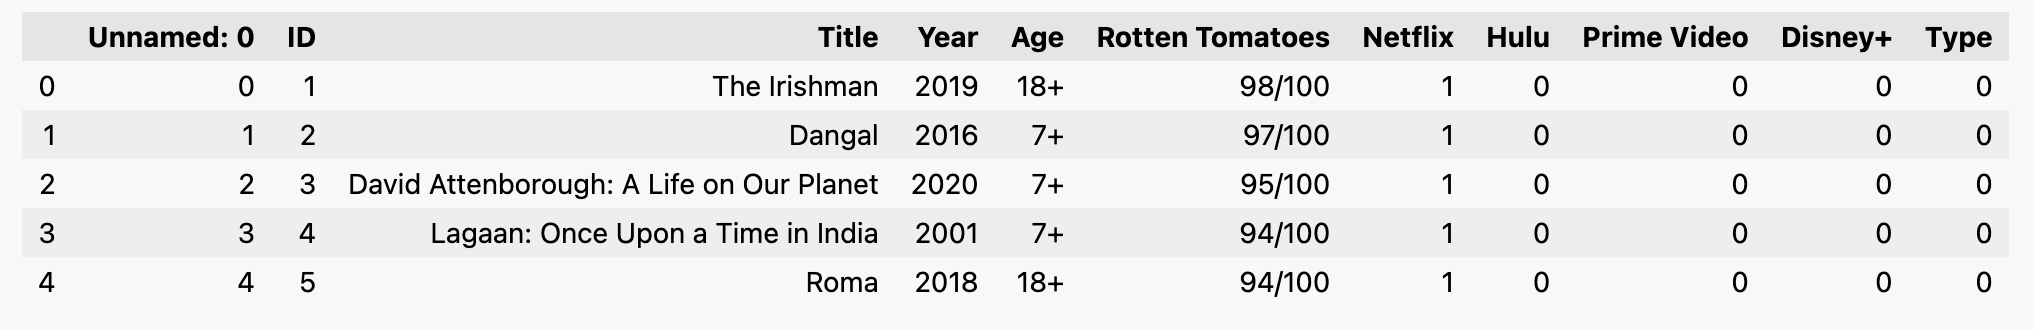
\includegraphics[width=1\textwidth]{head.png} % Replace with your image file
    \caption{First 5 Records of the Dataset}
    \label{fig:datatable}
\end{figure}

\subsection{Box Plot} \label{appendix:box_plot}
A box plot, or whisker plot, visualizes a dataset’s distribution, showing its central tendency, spread, and outliers \cite{mcgill1978boxplots}.

\begin{enumerate}
    \item \textbf{Median (\(Q2\))}: 
    The midpoint of the dataset, dividing it into two equal halves:
    \[
    Q2 = 
    \begin{cases} 
    x_{\left(\frac{n+1}{2}\right)} & \text{if } n \text{ is odd} \\
    \frac{x_{\left(\frac{n}{2}\right)} + x_{\left(\frac{n}{2}+1\right)}}{2} & \text{if } n \text{ is even}.
    \end{cases}
    \]
    \item \textbf{Interquartile Range (IQR)}:
    The range of the middle 50\% of the data:
    \[
    IQR = Q3 - Q1
    \]
    where \(Q1\) and \(Q3\) are the 25th and 75th percentiles, respectively.

    \item \textbf{Whiskers}:
    Extend to the smallest and largest values within 1.5 times the IQR:
    \[
    \text{Lower whisker} = \max(\min(\text{data}), Q1 - 1.5 \times IQR)
    \]
    \[
    \text{Upper whisker} = \min(\max(\text{data}), Q3 + 1.5 \times IQR)
    \]

    \item \textbf{Outliers}:
    Data points beyond the whiskers:
    \[
    \text{Outliers} < Q1 - 1.5 \times IQR \quad \text{or} \quad \text{Outliers} > Q3 + 1.5 \times IQR.
    \]
\end{enumerate}

Box plots help identify the \textbf{median} (central tendency), \textbf{IQR} (spread), and \textbf{outliers} (anomalies).


\subsection{Shapiro-Wilk Test} \label{appendix:shapiro}
The Shapiro-Wilk test evaluates whether a dataset follows a normal distribution. It calculates a test statistic based on the correlation between the data and their corresponding normal scores. The test statistic \(W\) is defined as:

\[
W = \frac{\left( \sum_{i=1}^{n} a_i x_{(i)} \right)^2}{\sum_{i=1}^{n} (x_i - \bar{x})^2}
\]

Where:
\begin{itemize}
    \item \(x_{(i)}\): Ordered sample values (from smallest to largest).
    \item \(a_i\): Weights derived from the expected values of the order statistics of a standard normal distribution.
    \item \(\bar{x}\): Sample mean.
    \item \(n\): Number of observations.
\end{itemize}

A \textbf{p-value $<$ 0.05} suggests that the data significantly deviate from normality. This test is particularly effective for small sample sizes. \cite{shapiro1965}

\subsection{Kolmogorov-Smirnov Test} \label{appendix:kolmogorov}
The Kolmogorov-Smirnov (K-S) test compares the empirical cumulative distribution function (ECDF) of a dataset, \(F_n(x)\), to a specified theoretical cumulative distribution function (CDF), \(F(x)\). The test statistic \(D\) is defined as:

\[
D = \max | F_n(x) - F(x) |
\]

Where:
\begin{itemize}
    \item \(F_n(x)\): Empirical CDF of the sample.
    \item \(F(x)\): Theoretical CDF of the specified distribution (e.g., normal).
\end{itemize}

A \textbf{p-value $<$ 0.05} indicates that the data do not follow the specified distribution. The test is sensitive to differences in both the center and the tails of the distribution. \cite{smirnov1948}

\subsection{Mann-Whitney U Test} \label{appendix:mann}
The \textbf{Mann-Whitney U test} is a non-parametric test used to determine whether there is a significant difference between the distributions of two independent groups. Unlike the t-test, it does not assume normality or equal variances. The test ranks all data points from both groups together and then evaluates whether the ranks of one group are systematically higher or lower than the other. It is particularly useful for comparing medians or when the data are ordinal or not normally distributed. \cite{mann1947}

\subsection{P-value} \label{appendix:pvalue}
The \textbf{p-value} is a measure used in statistical hypothesis testing to quantify the evidence against the null hypothesis (\(H_0\)). It represents the probability of observing a test statistic as extreme as, or more extreme than, the one observed, assuming that \(H_0\) is true.

Mathematically, the p-value is defined as:
\[
p = P(T \geq T_{\text{obs}} \mid H_0)
\]
where:
\begin{itemize}
    \item \(T\) is the test statistic.
    \item \(T_{\text{obs}}\) is the observed value of the test statistic.
    \item \(H_0\) is the null hypothesis.
\end{itemize}

A smaller p-value (e.g., \(p < 0.05\)) indicates stronger evidence against the null hypothesis, leading to its rejection. Conversely, a larger p-value suggests insufficient evidence to reject \(H_0\). \cite{pearson1900}


\end{document}
